\documentclass[10pt,letterpaper]{article}
\usepackage[top=1in,left=1in,right=1in, bottom=1in]{geometry}

% amsmath and amssymb packages, useful for mathematical formulas and symbols
\usepackage{amsmath,amssymb}

% textcomp package and marvosym package for additional characters
\usepackage{textcomp,marvosym}

\bibliographystyle{plos2015}


% line numbers
\usepackage[right]{lineno}

% easier turning on/off of includegraphics
\usepackage{ifthen}
\newboolean{includefigs}
\setboolean{includefigs}{true} % true/false

% ligatures disabled
\usepackage[nopatch=eqnum]{microtype}
\DisableLigatures[f]{encoding = *, family = * }

% Bold the 'Figure #' in the caption and separate it from the title/caption with a period
% Captions will be left justified
\usepackage[aboveskip=1pt,labelfont=bf,labelsep=period,justification=raggedright,singlelinecheck=off]{caption}
\renewcommand{\figurename}{Fig}
\renewcommand{\thefigure}{S.G.\arabic{figure}}
\renewcommand{\thetable}{S.G.\arabic{table}}


% create \thickcline for thick horizontal lines of variable length
\newlength\savedwidth
\newcommand\thickcline[1]{%
  \noalign{\global\savedwidth\arrayrulewidth\global\arrayrulewidth 2pt}%
  \cline{#1}%
  \noalign{\vskip\arrayrulewidth}%
  \noalign{\global\arrayrulewidth\savedwidth}%
}

% \thickhline command for thick horizontal lines that span the table
\newcommand\thickhline{\noalign{\global\savedwidth\arrayrulewidth\global\arrayrulewidth 2pt}%
\hline
\noalign{\global\arrayrulewidth\savedwidth}}

% Remove this for final submission, do not include graphics
\usepackage{graphicx} % Required for inserting images


% Use nameref to cite supporting information files (see Supporting Information section for more info)
\usepackage{nameref,hyperref}


\usepackage{datatool}
\DTLsetseparator{,}% Set the separator between the columns.
% todo add statistics file directly into this document
\DTLloaddbtex{\mydata}{../../output/statistics.dbtex}
\newcommand{\var}[1]{\DTLfetch{\mydata}{labels}{#1}{vals}}


\title{Quantifying prevalence and risk factors of HIV multiple infection in Uganda from population-based deep-sequence data}

\begin{document}
%TITLE_VPSACE

% Title must be 250 characters or less.
\begin{flushleft}

{\Large\textbf\newline{Quantifying prevalence and risk factors of HIV multiple infection in Uganda from population-based deep-sequence data \\ \medskip \large Supplementary File 5: Sensitivity of results to choice of genome windows} 
%
%
% Please use "sentence case" for title and headings (capitalize only the first word in a title (or heading), the first word in a subtitle (or subheading), and any proper nouns).
}
\newline
% Insert author names, affiliations and corresponding author email (do not include titles, positions, or degrees).
\\
Michael A. Martin\textsuperscript{1,$\dagger$},
Andrea Brizzi\textsuperscript{2},
Xiaoyue Xi\textsuperscript{2,3},
Ronald Moses Galiwango\textsuperscript{4},
Sikhulile Moyo\textsuperscript{5,6},
Deogratius Ssemwanga\textsuperscript{7,8}
Alexandra Blenkinsop\textsuperscript{2},
Andrew D. Redd\textsuperscript{9,10,11},
Lucie Abeler-Dörner\textsuperscript{12},
Christophe Fraser\textsuperscript{12},
Steven J. Reynolds\textsuperscript{4,9,10},
Thomas C. Quinn\textsuperscript{4,9,10},
Joseph Kagaayi\textsuperscript{4,13},
David Bonsall\textsuperscript{14},
David Serwadda\textsuperscript{4},
Gertrude Nakigozi\textsuperscript{4},
Godfrey Kigozi\textsuperscript{4},
M. Kate Grabowski\textsuperscript{1,4,15,$\dagger$},
Oliver Ratmann\textsuperscript{2,$\dagger$},
with the PANGEA-HIV Consortium and the Rakai Health Sciences Program
\\
\bigskip
\textbf{1} Department of Pathology, Johns Hopkins School of Medicine, Baltimore, MD, USA
\\
\textbf{2} Department of Mathematics, Imperial College London, London, United Kingdom
\\
\textbf{3} Medical Research Council Biostatistics Unit, University of Cambridge, Cambridge, UK \\

\textbf{4} Rakai Health Sciences Program, Kalisizo, Uganda \\

\textbf{5} Botswana Harvard AIDS Institute Partnership, Botswana Harvard HIV Reference Laboratory, Gaborone, Botswana \\

\textbf{6} Harvard T.H. Chan School of Public Health, Boston, MA, USA \\

\textbf{7} Medical Research Council/Uganda Virus Research Institute and London School of Hygiene and Tropical Medicine Uganda Research Unit, Entebbe, Uganda \\

\textbf{8} Uganda Virus Research Institute, Entebbe, Uganda \\

\textbf{9} Department of Medicine, Johns Hopkins School of Medicine, Baltimore, MD, USA
\\
\textbf{10} Division of Intramural Research, National Institute of Allergy and Infectious Diseases, National Institutes of Health, Bethesda, MD, USA
\\
\textbf{11} Institute of Infectious Disease and Molecular Medicine, University of Cape Town, Cape Town, South Africa
\\
\textbf{12} Pandemic Sciences Institute, Nuffield Department of Medicine, University of Oxford, Oxford, UK \\

\textbf{13} Makerere University School of Public Health, Kampala, Uganda \\

\textbf{14} Wellcome Centre for Human Genetics, Nuffield Department of Medicine, University of Oxford, Oxford, UK \\

\textbf{15} Department of Epidemiology, Johns Hopkins Bloomberg School of Public Health, Baltimore, MD, USA \\

\bigskip
% Use the asterisk to denote corresponding authorship and provide email address in note below.
$\dagger$ Corresponding authors mmart108@jhmi.edu, mgrabow2@jhu.edu, oliver.ratmann@imperial.ac.uk 
\end{flushleft}

\section{Choice of genome window}
Phylogenetic trees from the HIV deep-sequence reads generated from \var{n_unique_N_obs_gt_0} Rakai Community Cohort Study participants living with viremic HIV using \textit{phyloscanner}. In total, phylogenetic trees were inferred using data from \var{n_all_windows} \var{phsc_window_size} base pair (bp) overlapping windows with a \var{phsc_step_size} bp step between windows. To generate a set of independent data points from each sequenced participant-visit we first downsampled the \var{n_all_windows} overlapping windows to a set of \var{n_unique_windows} \var{phsc_window_size} bp windows beginning at position 800 in the HXB2 (GenBank: K03455.1) genome.  Summarized data in the form of the genome coverage in the phyloscanner output ($N^{obs}_i$) and the number of windows with multiple phylogenetic subgraphs ($MI^{obs}_i$) was highly correlated between the set of full windows and the set of non-overlapping windows (Pearson's $\rho=$ \var{all_unique_n_corr}, \var{all_unique_mi_corr}, respectively, Genome Window Fig~\ref{all_uniq_corr}). \par
Additionally, we simulate synthetic amplicon data by selecting data from \textit{phyloscanner} windows spanning the \textit{p24} and \textit{gp41} regions of the HIV genome. Specifically, we aim to generate data covering nucleotides 1,427 through 1,816 (\textit{p24}) and 7,941 through 8,264 (\textit{gp41}) of HXB2 based on the amplicons used for earlier studies of HIV multiple infection \cite{redd2011, redd2012, redd2014}. As these regions are larger than our 250 bp \textit{phyloscanner} windows we first take data from the fist and the last window that are entirely contained within each target region. Sequenced participant-visits were assigned $N^\text{obs}_{i,r} = 1$ (where $r$ indicates the amplicon region) in each region if $N^\text{obs}_{i,w} = 1$ for both of the selected windows in a given amplicon region. We set $MI^\text{obs}_{i,r} = 1$ if $MI^\text{obs}_{i,w} =1 $ in either of the selected windows spanning a given amplicon region. 

\begin{figure}[!ht]
 \ifthenelse{\boolean{includefigs}}{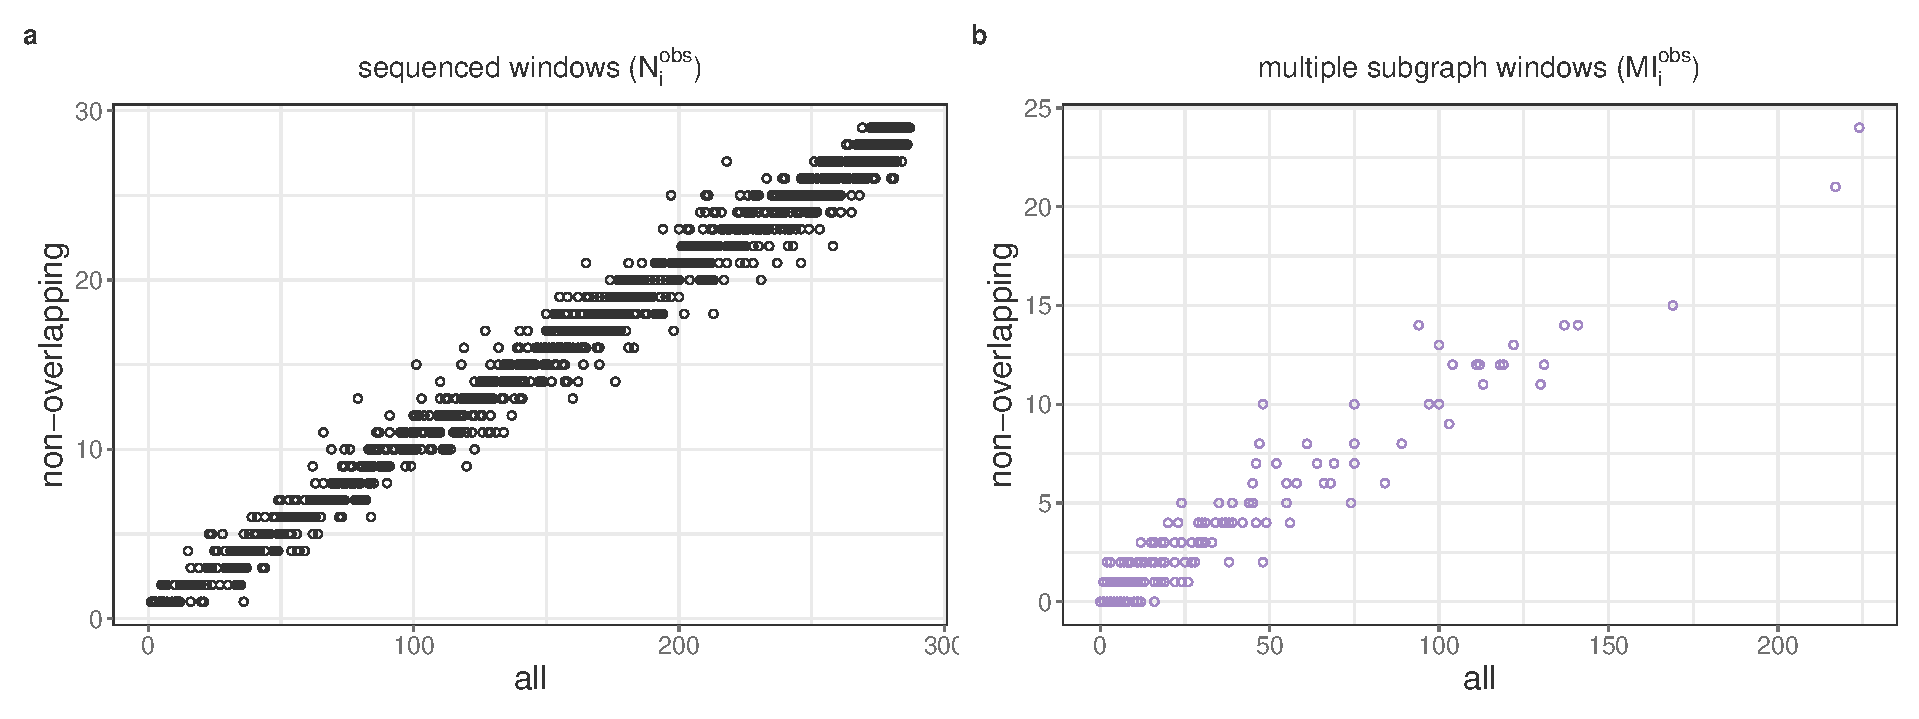
\includegraphics[width=1\textwidth]{../../figures/all_uniq_corr.pdf}}{}
\caption{{\bf Correlation between summary statistics from within-host deep sequence phylogenies from all genome windows and non-overlapping windows generated from \protect \var{n_unique_N_obs_gt_0} Rakai Community Cohort Study living with viremic HIV.} (A) Number of windows with phyloscanner output for each participant-visit. (B) Number of windows with multiple phylogenetic subgraphs for each participant-visit.}
\label{all_uniq_corr}
\end{figure}


\section{Alternate set of non-overlapping windows}
Based on the window size and window step size, there are 10 potential sets of non-overlapping windows that could have been chosen to generate a set of independent data-points for each sequenced participant visits. To assess the sensitivity of our results to the choice of non-overlapping windows we alternatively downsampled the data to the set of non-overlapping \var{phsc_window_size} bp windows beginning at position 950 in the HXB2 genome. Genome coverage and the number of windows with multiple phylogenetic subgraphs was highly correlated between the two sets of non-overlapping windows (Pearson's $\rho=$ \var{unique_unique_alt_n_corr}, \var{unique_unique_alt_mi_corr}, respectively).

\begin{figure}[!ht]
 \ifthenelse{\boolean{includefigs}}{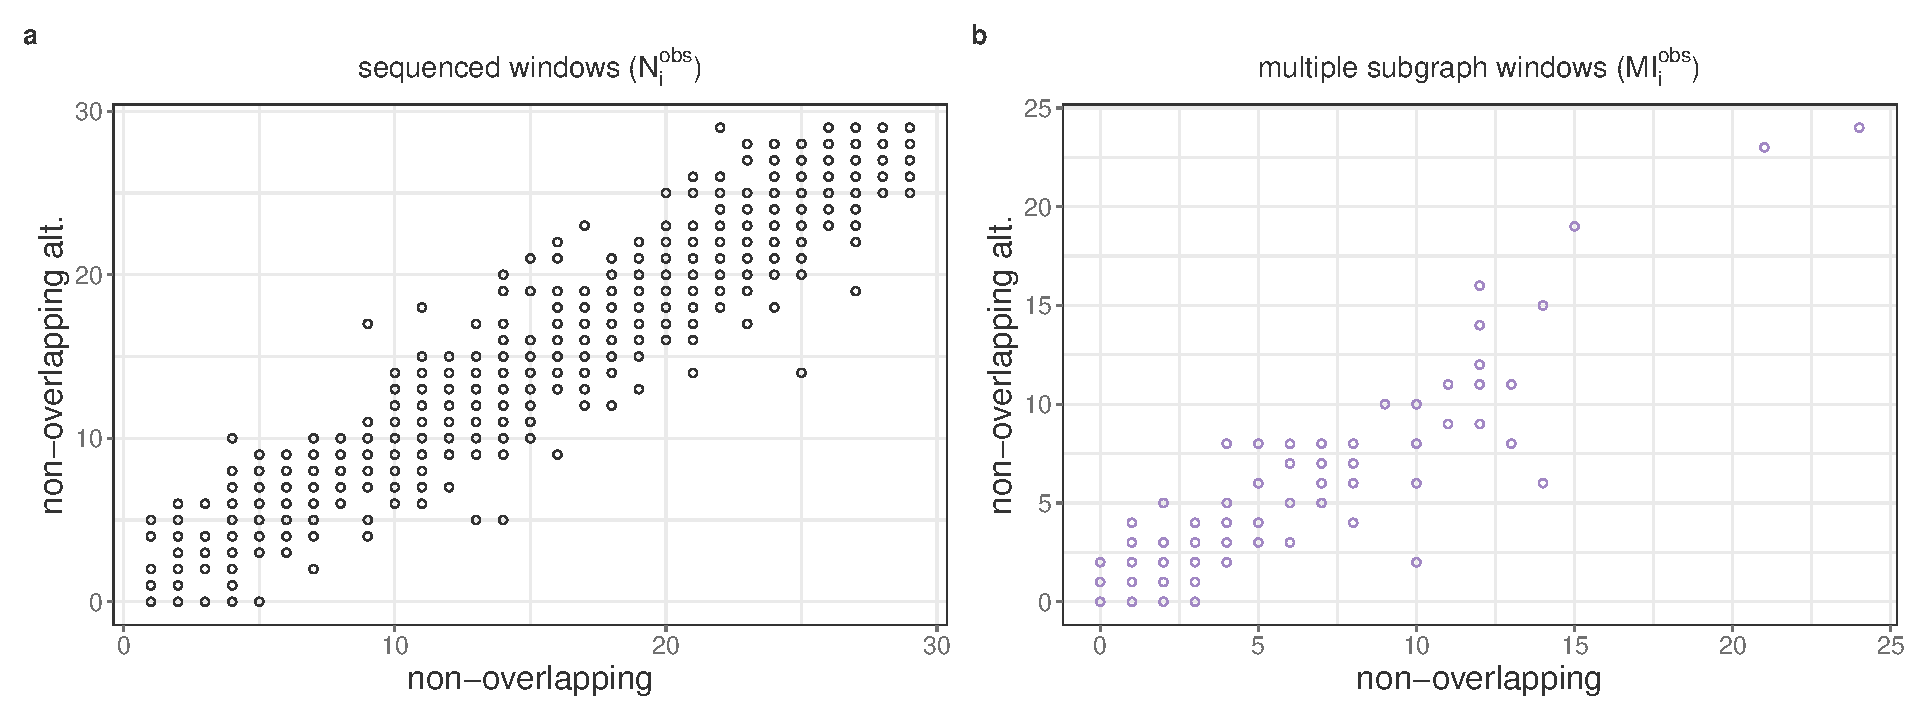
\includegraphics[width=1\textwidth]{../../figures/uniq_uniq_alt_corr.pdf}}{}
\caption{{\bf Correlation between summary statistics from within-host deep sequence phylogenies from all genome windows and non-overlapping windows generated from \protect \var{n_unique_N_obs_gt_0} Rakai Community Cohort Study participant-visits living with viremic HIV.} (A) Number of windows with phyloscanner output for each participant-visit. (B) Number of windows with multiple phylogenetic subgraphs for each participant-visit.}
\label{uniq_uniq_alt_corr}
\end{figure}

\section{Sensitivity of results to non-overlapping windows}
Finally, we fit our inference model accounting for partial sequencing success, false negative multiple subgraph windows, and false positive multiple subgraph windows to data from the two sets of non-overlapping genome windows (Table~\ref{empirical_age_sex_comm_table}-\ref{empirical_age_sex_comm_alt_table}). We note that parameter estimates from the two model fits are highly similar, indicating that our results are not particularly sensitive to the exact choice of genome window sets. 


\begin{table}[hbp!]
%\begin{adjustwidth}{-2.25in}{0in} % Comment out/remove adjustwidth environment if table fits in text column.
\centering
\begin{tabular}[t]{|l|c|c|c|c|c|}
\hline
Parameter & Prior & Median (95\% HPD) & Bulk ESS & Tail ESS & $\hat{R}$ \\ \thickhline
$\alpha_0$ & Normal(0,$2^2$) &
  \var{empirical_age_sex_comm_fit_logit_prob_seq_baseline_median} 
    (\var{empirical_age_sex_comm_fit_logit_prob_seq_baseline_lower}, \var{empirical_age_sex_comm_fit_logit_prob_seq_baseline_upper}) & 
  \var{empirical_age_sex_comm_fit_logit_prob_seq_baseline_bulk_ess} & 
  \var{empirical_age_sex_comm_fit_logit_prob_seq_baseline_tail_ess} & 
  \var{empirical_age_sex_comm_fit_logit_prob_seq_baseline_rhat} \\ \hline
$\alpha_1$ (amplicon) & $2\times\text{stz-MVN}_1(0,1)$
 &
  \var{empirical_age_sex_comm_fit_logit_prob_seq_coeffs1_median}
    (\var{empirical_age_sex_comm_fit_logit_prob_seq_coeffs1_lower}, \var{empirical_age_sex_comm_fit_logit_prob_seq_coeffs1_upper}) & 
  \var{empirical_age_sex_comm_fit_logit_prob_seq_coeffs1_bulk_ess} & 
  \var{empirical_age_sex_comm_fit_logit_prob_seq_coeffs1_tail_ess} & 
  \var{empirical_age_sex_comm_fit_logit_prob_seq_coeffs1_rhat} \\ \hline
$\alpha_2$ (bait-capture) & $2\times\text{stz-MVN}_1(0,1)$ &
  \var{empirical_age_sex_comm_fit_logit_prob_seq_coeffs2_median}
    (\var{empirical_age_sex_comm_fit_logit_prob_seq_coeffs2_lower}, \var{empirical_age_sex_comm_fit_logit_prob_seq_coeffs2_upper}) & 
  \var{empirical_age_sex_comm_fit_logit_prob_seq_coeffs2_bulk_ess} & 
  \var{empirical_age_sex_comm_fit_logit_prob_seq_coeffs2_tail_ess} & 
  \var{empirical_age_sex_comm_fit_logit_prob_seq_coeffs2_rhat} \\ \hline
$\alpha_3$ (log$_{10}$ copies/mL) & Normal(0,$2^2$) &
  \var{empirical_age_sex_comm_fit_logit_prob_seq_coeffs3_median}
    (\var{empirical_age_sex_comm_fit_logit_prob_seq_coeffs3_lower}, \var{empirical_age_sex_comm_fit_logit_prob_seq_coeffs3_upper}) & 
  \var{empirical_age_sex_comm_fit_logit_prob_seq_coeffs3_bulk_ess} & 
  \var{empirical_age_sex_comm_fit_logit_prob_seq_coeffs3_tail_ess} & 
  \var{empirical_age_sex_comm_fit_logit_prob_seq_coeffs3_rhat} \\ \hline

$\alpha_4$ (amplicon $\times$ log$_{10}$ copies/mL) & $2\times\text{stz-MVN}_2(0,1)$ &
  \var{empirical_age_sex_comm_fit_logit_prob_seq_coeffs4_median}
    (\var{empirical_age_sex_comm_fit_logit_prob_seq_coeffs4_lower}, \var{empirical_age_sex_comm_fit_logit_prob_seq_coeffs4_upper}) & 
  \var{empirical_age_sex_comm_fit_logit_prob_seq_coeffs4_bulk_ess} & 
  \var{empirical_age_sex_comm_fit_logit_prob_seq_coeffs4_tail_ess} & 
  \var{empirical_age_sex_comm_fit_logit_prob_seq_coeffs4_rhat} \\ \hline


$\alpha_4$ (bait-capture $\times$ log$_{10}$ copies/mL) & $2\times\text{stz-MVN}_2(0,1)$ &
  \var{empirical_age_sex_comm_fit_logit_prob_seq_coeffs5_median}
    (\var{empirical_age_sex_comm_fit_logit_prob_seq_coeffs5_lower}, \var{empirical_age_sex_comm_fit_logit_prob_seq_coeffs5_upper}) & 
  \var{empirical_age_sex_comm_fit_logit_prob_seq_coeffs5_bulk_ess} & 
  \var{empirical_age_sex_comm_fit_logit_prob_seq_coeffs5_tail_ess} & 
  \var{empirical_age_sex_comm_fit_logit_prob_seq_coeffs5_rhat} \\ \hline
$\sigma_\alpha$ & Half-Cauchy(0,1) & 
  \var{empirical_age_sex_comm_fit_logit_prob_seq_ind_sd_median}
    (\var{empirical_age_sex_comm_fit_logit_prob_seq_ind_sd_lower}, \var{empirical_age_sex_comm_fit_logit_prob_seq_ind_sd_upper}) & 
  \var{empirical_age_sex_comm_fit_logit_prob_seq_ind_sd_bulk_ess} & 
  \var{empirical_age_sex_comm_fit_logit_prob_seq_ind_sd_tail_ess} &
  \var{empirical_age_sex_comm_fit_logit_prob_seq_ind_sd_rhat} \\ \hline
$\delta_0$ & Normal(0,$3.16^2$) &
  \var{empirical_age_sex_comm_fit_logit_prob_mi_baseline_median}
    (\var{empirical_age_sex_comm_fit_logit_prob_mi_baseline_lower}, \var{empirical_age_sex_comm_fit_logit_prob_mi_baseline_upper}) & 
  \var{empirical_age_sex_comm_fit_logit_prob_mi_baseline_bulk_ess} & 
  \var{empirical_age_sex_comm_fit_logit_prob_mi_baseline_tail_ess} & 
  \var{empirical_age_sex_comm_fit_logit_prob_mi_baseline_rhat} \\ \hline
$\beta_1$ ((14,24] years) & $\text{stz-MVN}_3(0,1)$ &  
  \var{empirical_age_sex_comm_fit_logit_prob_mi_coeffs1_median}
    (\var{empirical_age_sex_comm_fit_logit_prob_mi_coeffs1_lower}, \var{empirical_age_sex_comm_fit_logit_prob_mi_coeffs1_upper}) & 
  \var{empirical_age_sex_comm_fit_logit_prob_mi_coeffs1_bulk_ess} & 
  \var{empirical_age_sex_comm_fit_logit_prob_mi_coeffs1_tail_ess} & 
  \var{empirical_age_sex_comm_fit_logit_prob_mi_coeffs1_rhat} \\ \hline
$\beta_2$ ((24,34] years)) & $\text{stz-MVN}_3(0,1)$ &  
  \var{empirical_age_sex_comm_fit_logit_prob_mi_coeffs2_median}
    (\var{empirical_age_sex_comm_fit_logit_prob_mi_coeffs2_lower}, \var{empirical_age_sex_comm_fit_logit_prob_mi_coeffs2_upper}) & 
  \var{empirical_age_sex_comm_fit_logit_prob_mi_coeffs2_bulk_ess} & 
  \var{empirical_age_sex_comm_fit_logit_prob_mi_coeffs2_tail_ess} & 
  \var{empirical_age_sex_comm_fit_logit_prob_mi_coeffs2_rhat} \\ \hline
$\beta_3$ ((34,49] years) & $\text{stz-MVN}_3(0,1)$ &  
  \var{empirical_age_sex_comm_fit_logit_prob_mi_coeffs3_median}
    (\var{empirical_age_sex_comm_fit_logit_prob_mi_coeffs3_lower}, \var{empirical_age_sex_comm_fit_logit_prob_mi_coeffs3_upper}) & 
  \var{empirical_age_sex_comm_fit_logit_prob_mi_coeffs3_bulk_ess} & 
  \var{empirical_age_sex_comm_fit_logit_prob_mi_coeffs3_tail_ess} & 
  \var{empirical_age_sex_comm_fit_logit_prob_mi_coeffs3_rhat} \\ \hline
$\beta_4$ (women) & $\text{stz-MVN}_4(0,1)$ &  
  \var{empirical_age_sex_comm_fit_logit_prob_mi_coeffs4_median}
    (\var{empirical_age_sex_comm_fit_logit_prob_mi_coeffs4_lower}, \var{empirical_age_sex_comm_fit_logit_prob_mi_coeffs4_upper}) & 
  \var{empirical_age_sex_comm_fit_logit_prob_mi_coeffs4_bulk_ess} & 
  \var{empirical_age_sex_comm_fit_logit_prob_mi_coeffs4_tail_ess} & 
  \var{empirical_age_sex_comm_fit_logit_prob_mi_coeffs4_rhat} \\ \hline

$\beta_5$ (men) & $\text{stz-MVN}_4(0,1)$ &  
  \var{empirical_age_sex_comm_fit_logit_prob_mi_coeffs5_median}
    (\var{empirical_age_sex_comm_fit_logit_prob_mi_coeffs5_lower}, \var{empirical_age_sex_comm_fit_logit_prob_mi_coeffs5_upper}) & 
  \var{empirical_age_sex_comm_fit_logit_prob_mi_coeffs5_bulk_ess} & 
  \var{empirical_age_sex_comm_fit_logit_prob_mi_coeffs5_tail_ess} & 
  \var{empirical_age_sex_comm_fit_logit_prob_mi_coeffs5_rhat} \\ \hline

$\beta_6$ (fishing) & $\text{stz-MVN}_5(0,1)$ &  
  \var{empirical_age_sex_comm_fit_logit_prob_mi_coeffs6_median}
    (\var{empirical_age_sex_comm_fit_logit_prob_mi_coeffs6_lower}, \var{empirical_age_sex_comm_fit_logit_prob_mi_coeffs6_upper}) & 
  \var{empirical_age_sex_comm_fit_logit_prob_mi_coeffs6_bulk_ess} & 
  \var{empirical_age_sex_comm_fit_logit_prob_mi_coeffs6_tail_ess} & 
  \var{empirical_age_sex_comm_fit_logit_prob_mi_coeffs6_rhat} \\ \hline

$\beta_7$ (inland) & $\text{stz-MVN}_5(0,1)$ &  
  \var{empirical_age_sex_comm_fit_logit_prob_mi_coeffs7_median}
    (\var{empirical_age_sex_comm_fit_logit_prob_mi_coeffs7_lower}, \var{empirical_age_sex_comm_fit_logit_prob_mi_coeffs7_upper}) & 
  \var{empirical_age_sex_comm_fit_logit_prob_mi_coeffs7_bulk_ess} & 
  \var{empirical_age_sex_comm_fit_logit_prob_mi_coeffs7_tail_ess} & 
  \var{empirical_age_sex_comm_fit_logit_prob_mi_coeffs7_rhat} \\ \hline
logit($\lambda$) & Normal(0,1)[,2.2] & 
  \var{empirical_age_sex_comm_fit_logit_prob_mi_fnr_median}
    (\var{empirical_age_sex_comm_fit_logit_prob_mi_fnr_lower}, \var{empirical_age_sex_comm_fit_logit_prob_mi_fnr_upper}) & 
  \var{empirical_age_sex_comm_fit_logit_prob_mi_fnr_bulk_ess} & 
  \var{empirical_age_sex_comm_fit_logit_prob_mi_fnr_tail_ess} & 
  \var{empirical_age_sex_comm_fit_logit_prob_mi_fnr_rhat} \\ \hline
logit($\epsilon$) & Normal(0,1) & 
  \var{empirical_age_sex_comm_fit_logit_prob_mi_fpr_median}
    (\var{empirical_age_sex_comm_fit_logit_prob_mi_fpr_lower}, \var{empirical_age_sex_comm_fit_logit_prob_mi_fpr_upper}) & 
  \var{empirical_age_sex_comm_fit_logit_prob_mi_fpr_bulk_ess} & 
  \var{empirical_age_sex_comm_fit_logit_prob_mi_fpr_tail_ess} & 
  \var{empirical_age_sex_comm_fit_logit_prob_mi_fpr_rhat} \\ \hline
\end{tabular}
\caption{{\bf Parameter estimates for full model fit to deep-sequence data from \protect \var{empirical_age_sex_comm_n_participant_visits} RCCS participants living with viremic HIV with age, sex, and community type as putative risk factors for harboring multiple infections.} ESS = effective sample size. HPD = highest posterior density. stz-MVN = sum-to-zero multivariate-Normal distribution. } 
\label{empirical_age_sex_comm_table}
\end{table}


\begin{table}[hbp!]
%\begin{adjustwidth}{-2.25in}{0in} % Comment out/remove adjustwidth environment if table fits in text column.
\centering
\begin{tabular}[t]{|l|c|c|c|c|c|}
\hline
Parameter & Prior & Median (95\% HPD) & Bulk ESS & Tail ESS & $\hat{R}$ \\ \thickhline

$\alpha_0$ & Normal(0,$2^2$) &
  \var{empirical_age_sex_comm_alt_fit_logit_prob_seq_baseline_median} 
    (\var{empirical_age_sex_comm_alt_fit_logit_prob_seq_baseline_lower}, \var{empirical_age_sex_comm_alt_fit_logit_prob_seq_baseline_upper}) & 
  \var{empirical_age_sex_comm_alt_fit_logit_prob_seq_baseline_bulk_ess} & 
  \var{empirical_age_sex_comm_alt_fit_logit_prob_seq_baseline_tail_ess} & 
  \var{empirical_age_sex_comm_alt_fit_logit_prob_seq_baseline_rhat} \\ \hline
$\alpha_1$ (amplicon) & $2\times\text{stz-MVN}_1(0,1)$ &
  \var{empirical_age_sex_comm_alt_fit_logit_prob_seq_coeffs1_median}
    (\var{empirical_age_sex_comm_alt_fit_logit_prob_seq_coeffs1_lower}, \var{empirical_age_sex_comm_alt_fit_logit_prob_seq_coeffs1_upper}) & 
  \var{empirical_age_sex_comm_alt_fit_logit_prob_seq_coeffs1_bulk_ess} & 
  \var{empirical_age_sex_comm_alt_fit_logit_prob_seq_coeffs1_tail_ess} & 
  \var{empirical_age_sex_comm_alt_fit_logit_prob_seq_coeffs1_rhat} \\ \hline
$\alpha_2$ (bait-capture) & $2\times\text{stz-MVN}_1(0,1)$ &
  \var{empirical_age_sex_comm_alt_fit_logit_prob_seq_coeffs2_median}
    (\var{empirical_age_sex_comm_alt_fit_logit_prob_seq_coeffs2_lower}, \var{empirical_age_sex_comm_alt_fit_logit_prob_seq_coeffs2_upper}) & 
  \var{empirical_age_sex_comm_alt_fit_logit_prob_seq_coeffs2_bulk_ess} & 
  \var{empirical_age_sex_comm_alt_fit_logit_prob_seq_coeffs2_tail_ess} & 
  \var{empirical_age_sex_comm_alt_fit_logit_prob_seq_coeffs2_rhat} \\ \hline
$\alpha_3$ (log$_{10}$ copies/mL) & Normal(0,$2^2$) &
  \var{empirical_age_sex_comm_alt_fit_logit_prob_seq_coeffs3_median}
    (\var{empirical_age_sex_comm_alt_fit_logit_prob_seq_coeffs3_lower}, \var{empirical_age_sex_comm_alt_fit_logit_prob_seq_coeffs3_upper}) & 
  \var{empirical_age_sex_comm_alt_fit_logit_prob_seq_coeffs3_bulk_ess} & 
  \var{empirical_age_sex_comm_alt_fit_logit_prob_seq_coeffs3_tail_ess} & 
  \var{empirical_age_sex_comm_alt_fit_logit_prob_seq_coeffs3_rhat} \\ \hline

$\alpha_4$ (amplicon $\times$ log$_{10}$ copies/mL) & $2\times\text{stz-MVN}_2(0,1)$&
  \var{empirical_age_sex_comm_alt_fit_logit_prob_seq_coeffs4_median}
    (\var{empirical_age_sex_comm_alt_fit_logit_prob_seq_coeffs4_lower}, \var{empirical_age_sex_comm_alt_fit_logit_prob_seq_coeffs4_upper}) & 
  \var{empirical_age_sex_comm_alt_fit_logit_prob_seq_coeffs4_bulk_ess} & 
  \var{empirical_age_sex_comm_alt_fit_logit_prob_seq_coeffs4_tail_ess} & 
  \var{empirical_age_sex_comm_alt_fit_logit_prob_seq_coeffs4_rhat} \\ \hline


$\alpha_4$ (bait-capture $\times$ log$_{10}$ copies/mL) & $2\times\text{stz-MVN}_2(0,1)$ &
  \var{empirical_age_sex_comm_alt_fit_logit_prob_seq_coeffs5_median}
    (\var{empirical_age_sex_comm_alt_fit_logit_prob_seq_coeffs5_lower}, \var{empirical_age_sex_comm_alt_fit_logit_prob_seq_coeffs5_upper}) & 
  \var{empirical_age_sex_comm_alt_fit_logit_prob_seq_coeffs5_bulk_ess} & 
  \var{empirical_age_sex_comm_alt_fit_logit_prob_seq_coeffs5_tail_ess} & 
  \var{empirical_age_sex_comm_alt_fit_logit_prob_seq_coeffs5_rhat} \\ \hline
$\sigma_\alpha$ & Half-Cauchy(0,1) & 
  \var{empirical_age_sex_comm_alt_fit_logit_prob_seq_ind_sd_median}
    (\var{empirical_age_sex_comm_alt_fit_logit_prob_seq_ind_sd_lower}, \var{empirical_age_sex_comm_alt_fit_logit_prob_seq_ind_sd_upper}) & 
  \var{empirical_age_sex_comm_alt_fit_logit_prob_seq_ind_sd_bulk_ess} & 
  \var{empirical_age_sex_comm_alt_fit_logit_prob_seq_ind_sd_tail_ess} &
  \var{empirical_age_sex_comm_alt_fit_logit_prob_seq_ind_sd_rhat} \\ \hline
$\delta_0$ & Normal(0,$3.16^2$) &
  \var{empirical_age_sex_comm_alt_fit_logit_prob_mi_baseline_median}
    (\var{empirical_age_sex_comm_alt_fit_logit_prob_mi_baseline_lower}, \var{empirical_age_sex_comm_alt_fit_logit_prob_mi_baseline_upper}) & 
  \var{empirical_age_sex_comm_alt_fit_logit_prob_mi_baseline_bulk_ess} & 
  \var{empirical_age_sex_comm_alt_fit_logit_prob_mi_baseline_tail_ess} & 
  \var{empirical_age_sex_comm_alt_fit_logit_prob_mi_baseline_rhat} \\ \hline
$\beta_1$ ((14,24] years) & $\text{stz-MVN}_3(0,1)$ &  
  \var{empirical_age_sex_comm_alt_fit_logit_prob_mi_coeffs1_median}
    (\var{empirical_age_sex_comm_alt_fit_logit_prob_mi_coeffs1_lower}, \var{empirical_age_sex_comm_alt_fit_logit_prob_mi_coeffs1_upper}) & 
  \var{empirical_age_sex_comm_alt_fit_logit_prob_mi_coeffs1_bulk_ess} & 
  \var{empirical_age_sex_comm_alt_fit_logit_prob_mi_coeffs1_tail_ess} & 
  \var{empirical_age_sex_comm_alt_fit_logit_prob_mi_coeffs1_rhat} \\ \hline
$\beta_2$ ((24,34] years)) & $\text{stz-MVN}_3(0,1)$ &  
  \var{empirical_age_sex_comm_alt_fit_logit_prob_mi_coeffs2_median}
    (\var{empirical_age_sex_comm_alt_fit_logit_prob_mi_coeffs2_lower}, \var{empirical_age_sex_comm_alt_fit_logit_prob_mi_coeffs2_upper}) & 
  \var{empirical_age_sex_comm_alt_fit_logit_prob_mi_coeffs2_bulk_ess} & 
  \var{empirical_age_sex_comm_alt_fit_logit_prob_mi_coeffs2_tail_ess} & 
  \var{empirical_age_sex_comm_alt_fit_logit_prob_mi_coeffs2_rhat} \\ \hline
$\beta_3$ ((34,49] years) & $\text{stz-MVN}_3(0,1)$ &  
  \var{empirical_age_sex_comm_alt_fit_logit_prob_mi_coeffs3_median}
    (\var{empirical_age_sex_comm_alt_fit_logit_prob_mi_coeffs3_lower}, \var{empirical_age_sex_comm_alt_fit_logit_prob_mi_coeffs3_upper}) & 
  \var{empirical_age_sex_comm_alt_fit_logit_prob_mi_coeffs3_bulk_ess} & 
  \var{empirical_age_sex_comm_alt_fit_logit_prob_mi_coeffs3_tail_ess} & 
  \var{empirical_age_sex_comm_alt_fit_logit_prob_mi_coeffs3_rhat} \\ \hline
$\beta_4$ (women) & $\text{stz-MVN}_4(0,1)$ &  
  \var{empirical_age_sex_comm_alt_fit_logit_prob_mi_coeffs4_median}
    (\var{empirical_age_sex_comm_alt_fit_logit_prob_mi_coeffs4_lower}, \var{empirical_age_sex_comm_alt_fit_logit_prob_mi_coeffs4_upper}) & 
  \var{empirical_age_sex_comm_alt_fit_logit_prob_mi_coeffs4_bulk_ess} & 
  \var{empirical_age_sex_comm_alt_fit_logit_prob_mi_coeffs4_tail_ess} & 
  \var{empirical_age_sex_comm_alt_fit_logit_prob_mi_coeffs4_rhat} \\ \hline

$\beta_5$ (men) &$\text{stz-MVN}_4(0,1)$&  
  \var{empirical_age_sex_comm_alt_fit_logit_prob_mi_coeffs5_median}
    (\var{empirical_age_sex_comm_alt_fit_logit_prob_mi_coeffs5_lower}, \var{empirical_age_sex_comm_alt_fit_logit_prob_mi_coeffs5_upper}) & 
  \var{empirical_age_sex_comm_alt_fit_logit_prob_mi_coeffs5_bulk_ess} & 
  \var{empirical_age_sex_comm_alt_fit_logit_prob_mi_coeffs5_tail_ess} & 
  \var{empirical_age_sex_comm_alt_fit_logit_prob_mi_coeffs5_rhat} \\ \hline

$\beta_6$ (fishing) &$\text{stz-MVN}_5(0,1)$ &  
  \var{empirical_age_sex_comm_alt_fit_logit_prob_mi_coeffs6_median}
    (\var{empirical_age_sex_comm_alt_fit_logit_prob_mi_coeffs6_lower}, \var{empirical_age_sex_comm_alt_fit_logit_prob_mi_coeffs6_upper}) & 
  \var{empirical_age_sex_comm_alt_fit_logit_prob_mi_coeffs6_bulk_ess} & 
  \var{empirical_age_sex_comm_alt_fit_logit_prob_mi_coeffs6_tail_ess} & 
  \var{empirical_age_sex_comm_alt_fit_logit_prob_mi_coeffs6_rhat} \\ \hline

$\beta_7$ (inland) & $\text{stz-MVN}_5(0,1)$ &  
  \var{empirical_age_sex_comm_alt_fit_logit_prob_mi_coeffs7_median}
    (\var{empirical_age_sex_comm_alt_fit_logit_prob_mi_coeffs7_lower}, \var{empirical_age_sex_comm_alt_fit_logit_prob_mi_coeffs7_upper}) & 
  \var{empirical_age_sex_comm_alt_fit_logit_prob_mi_coeffs7_bulk_ess} & 
  \var{empirical_age_sex_comm_alt_fit_logit_prob_mi_coeffs7_tail_ess} & 
  \var{empirical_age_sex_comm_alt_fit_logit_prob_mi_coeffs7_rhat} \\ \hline
logit($\lambda$) & Normal(0,1)[,2.2] & 
  \var{empirical_age_sex_comm_alt_fit_logit_prob_mi_fnr_median}
    (\var{empirical_age_sex_comm_alt_fit_logit_prob_mi_fnr_lower}, \var{empirical_age_sex_comm_alt_fit_logit_prob_mi_fnr_upper}) & 
  \var{empirical_age_sex_comm_alt_fit_logit_prob_mi_fnr_bulk_ess} & 
  \var{empirical_age_sex_comm_alt_fit_logit_prob_mi_fnr_tail_ess} & 
  \var{empirical_age_sex_comm_alt_fit_logit_prob_mi_fnr_rhat} \\ \hline
logit($\epsilon$) & Normal(0,1) & 
  \var{empirical_age_sex_comm_alt_fit_logit_prob_mi_fpr_median}
    (\var{empirical_age_sex_comm_alt_fit_logit_prob_mi_fpr_lower}, \var{empirical_age_sex_comm_alt_fit_logit_prob_mi_fpr_upper}) & 
  \var{empirical_age_sex_comm_alt_fit_logit_prob_mi_fpr_bulk_ess} & 
  \var{empirical_age_sex_comm_alt_fit_logit_prob_mi_fpr_tail_ess} & 
  \var{empirical_age_sex_comm_alt_fit_logit_prob_mi_fpr_rhat} \\ \hline
\end{tabular}
\caption{{\bf Parameter estimates for full model fit to deep-sequence data from \protect \var{empirical_age_sex_comm_n_participant_visits} RCCS participants living with viremic HIV with age, sex, and community type as putative risk factors for harboring multiple infections using alternative non-overlapping windows.} ESS = effective sample size. HPD = highest posterior density. stz-MVN = sum-to-zero multivariate-Normal distribution. } 
\label{empirical_age_sex_comm_alt_table}
\end{table}


\newpage

\linespread{1}
\bibliography{references.bib}
\end{document}